\documentclass[11pt,xcolor=svgnames]{beamer}
\usepackage{dsfont,natbib,setspace,changepage,multirow,times}
\mode<presentation>

% replaces beamer foot with simple page number
\setbeamertemplate{navigation symbols}{}
\setbeamercolor{frametitle}{fg=black}
\newcommand{\theme}{\color{Maroon}}

\setbeamertemplate{footline}{
   \raisebox{5pt}{\makebox[\paperwidth]{\hfill\makebox[20pt]{\color{gray}\scriptsize\insertframenumber}}}}

\usepackage{tikz}
  
\graphicspath{{../graphs/}}

\setbeamercolor{whitebox}{bg=gray!10}

% colors
\newcommand{\bk}{\color{black}}
\newcommand{\rd}{\color{red}}
\newcommand{\fg}{\color{ForestGreen}}
\newcommand{\bl}{\color{blue}}
\newcommand{\gr}{\color{black!60}}
\newcommand{\sg}{\color{DarkSlateGray}}
\newcommand{\br}{\color{SaddleBrown}}
\newcommand{\nv}{\color{Navy}}


% common math markups
\newcommand{\bs}[1]{\boldsymbol{#1}}
\newcommand{\mc}[1]{\mathcal{#1}}
\newcommand{\mr}[1]{\mathrm{#1}}
\newcommand{\bm}[1]{\mathbf{#1}}
\newcommand{\ds}[1]{\mathds{#1}}
\newcommand{\indep}{\perp\!\!\!\perp}

% spacing and style shorthand
\setstretch{1.1}

% shorthand
\newcommand{\sk}{\vspace{.5cm}}
\newcommand{\R}[1]{{\tt \nv #1}}
\newcommand{\til}{{\footnotesize$\bs{\stackrel{\sim}{}}$}}
\DeclareSymbolFont{extraup}{U}{zavm}{m}{n}
\DeclareMathSymbol{\vardiamond}{\mathalpha}{extraup}{87}

\begin{document}

\setcounter{page}{0}
{ \usebackgroundtemplate{
\includegraphics[height=\paperheight]{phoenix}}
\begin{frame}[plain]
\begin{center}


{\bf \Large [8] Big Data: Factor Models}

\vskip 1.5cm 
Matt Taddy, University of Chicago Booth School of Business

\vskip .2cm 
\texttt{faculty.chicagobooth.edu/matt.taddy/teaching} 


\end{center}
\end{frame} }


\begin{frame}


{Today is all about \theme  Dimension Reduction} \gr (more than
normal) 

\sk\bk
{\nv The setting:}  we have a high-dimensional matrix of data $\bm{X}$.\\

We'd like to reduce this to a function few  `important' factors.


\sk
We'll do this by building a simple linear model for $\bm{X}$ 
and \\use this model to represent $\bm{X}$ in a  lower dimensional
space.

\sk\sg
Factor modeling is a super useful framework,
whether you get a deep understanding or just learn how they work in practice.
\gr We'll cover a variety of ways to understand.

\end{frame}


\begin{frame}

{\bf \theme Factor Models \bk are parsimonious models for $\bm{X}$}

\sk
A factor model is regression for multivariate $\bm{x} = [x_1
\ldots x_p]$.
\[
\ds{E}[x_{ij}] = \varphi_{j1} v_{i1} + \ldots  \varphi_{jK} v_{iK}, ~~i=1..n,~j=1..p
\]
The $v_{ik}$'s
are shared by all $p$ dimensions of $\bm{x}_i$, \\and the $\varphi_{jk}$
are the same for all $n$ observations.

\sk
 For example\\
~~~~~~~single factor: $\ds{E}[\bm{x}_i] = \bs{\varphi}v_i$\\ 
~~~~~~~two
factors: $\ds{E}[\bm{x}_i] = \bs{\varphi}_1v_{i1} + \bs{\varphi}_2v_{i2}$


\sk
The $\varphi_{jk}$ coefficients are called `{\nv loadings}' or `{\nv rotations}'. \\They are just
coefficients for regression of $\bm{x}_i$ onto $\bm{v}_i$.

\end{frame}

\begin{frame}

{\bf \theme Factor Models: \bk 
$
\ds{E}[\bm{ x}_{i}] = \bs{\varphi}_{1} v_{i1} + \ldots  \bs{\varphi}_{K} v_{iK}$}


\sk\gr
Each observation has $K$ factors $v_1 \ldots v_K$.  \bk
Since usually $K < p$, these factors are a lower dimension
  simplification of $\bm{x}$.

\sk
\gr
Each factor $v_{ik}$ is a univariate variable, and $\bm{v}_i =
[v_{i1} \ldots v_{iK}]$.\\\bk  The loadings
are $p$-dimensional, and they translate from the simple
(length-$K$) factor $\bm{v}_i$ to the complex (length-$p$) $\bm{x}_i$.

\sk
You can either treat the factors as unknown (PCA) \\or use $y$
 to build  them (PLS).
\end{frame}

\begin{frame}

{\bf \theme Geo-Genes Example: \bk two interpretable factors.}

\begin{center}
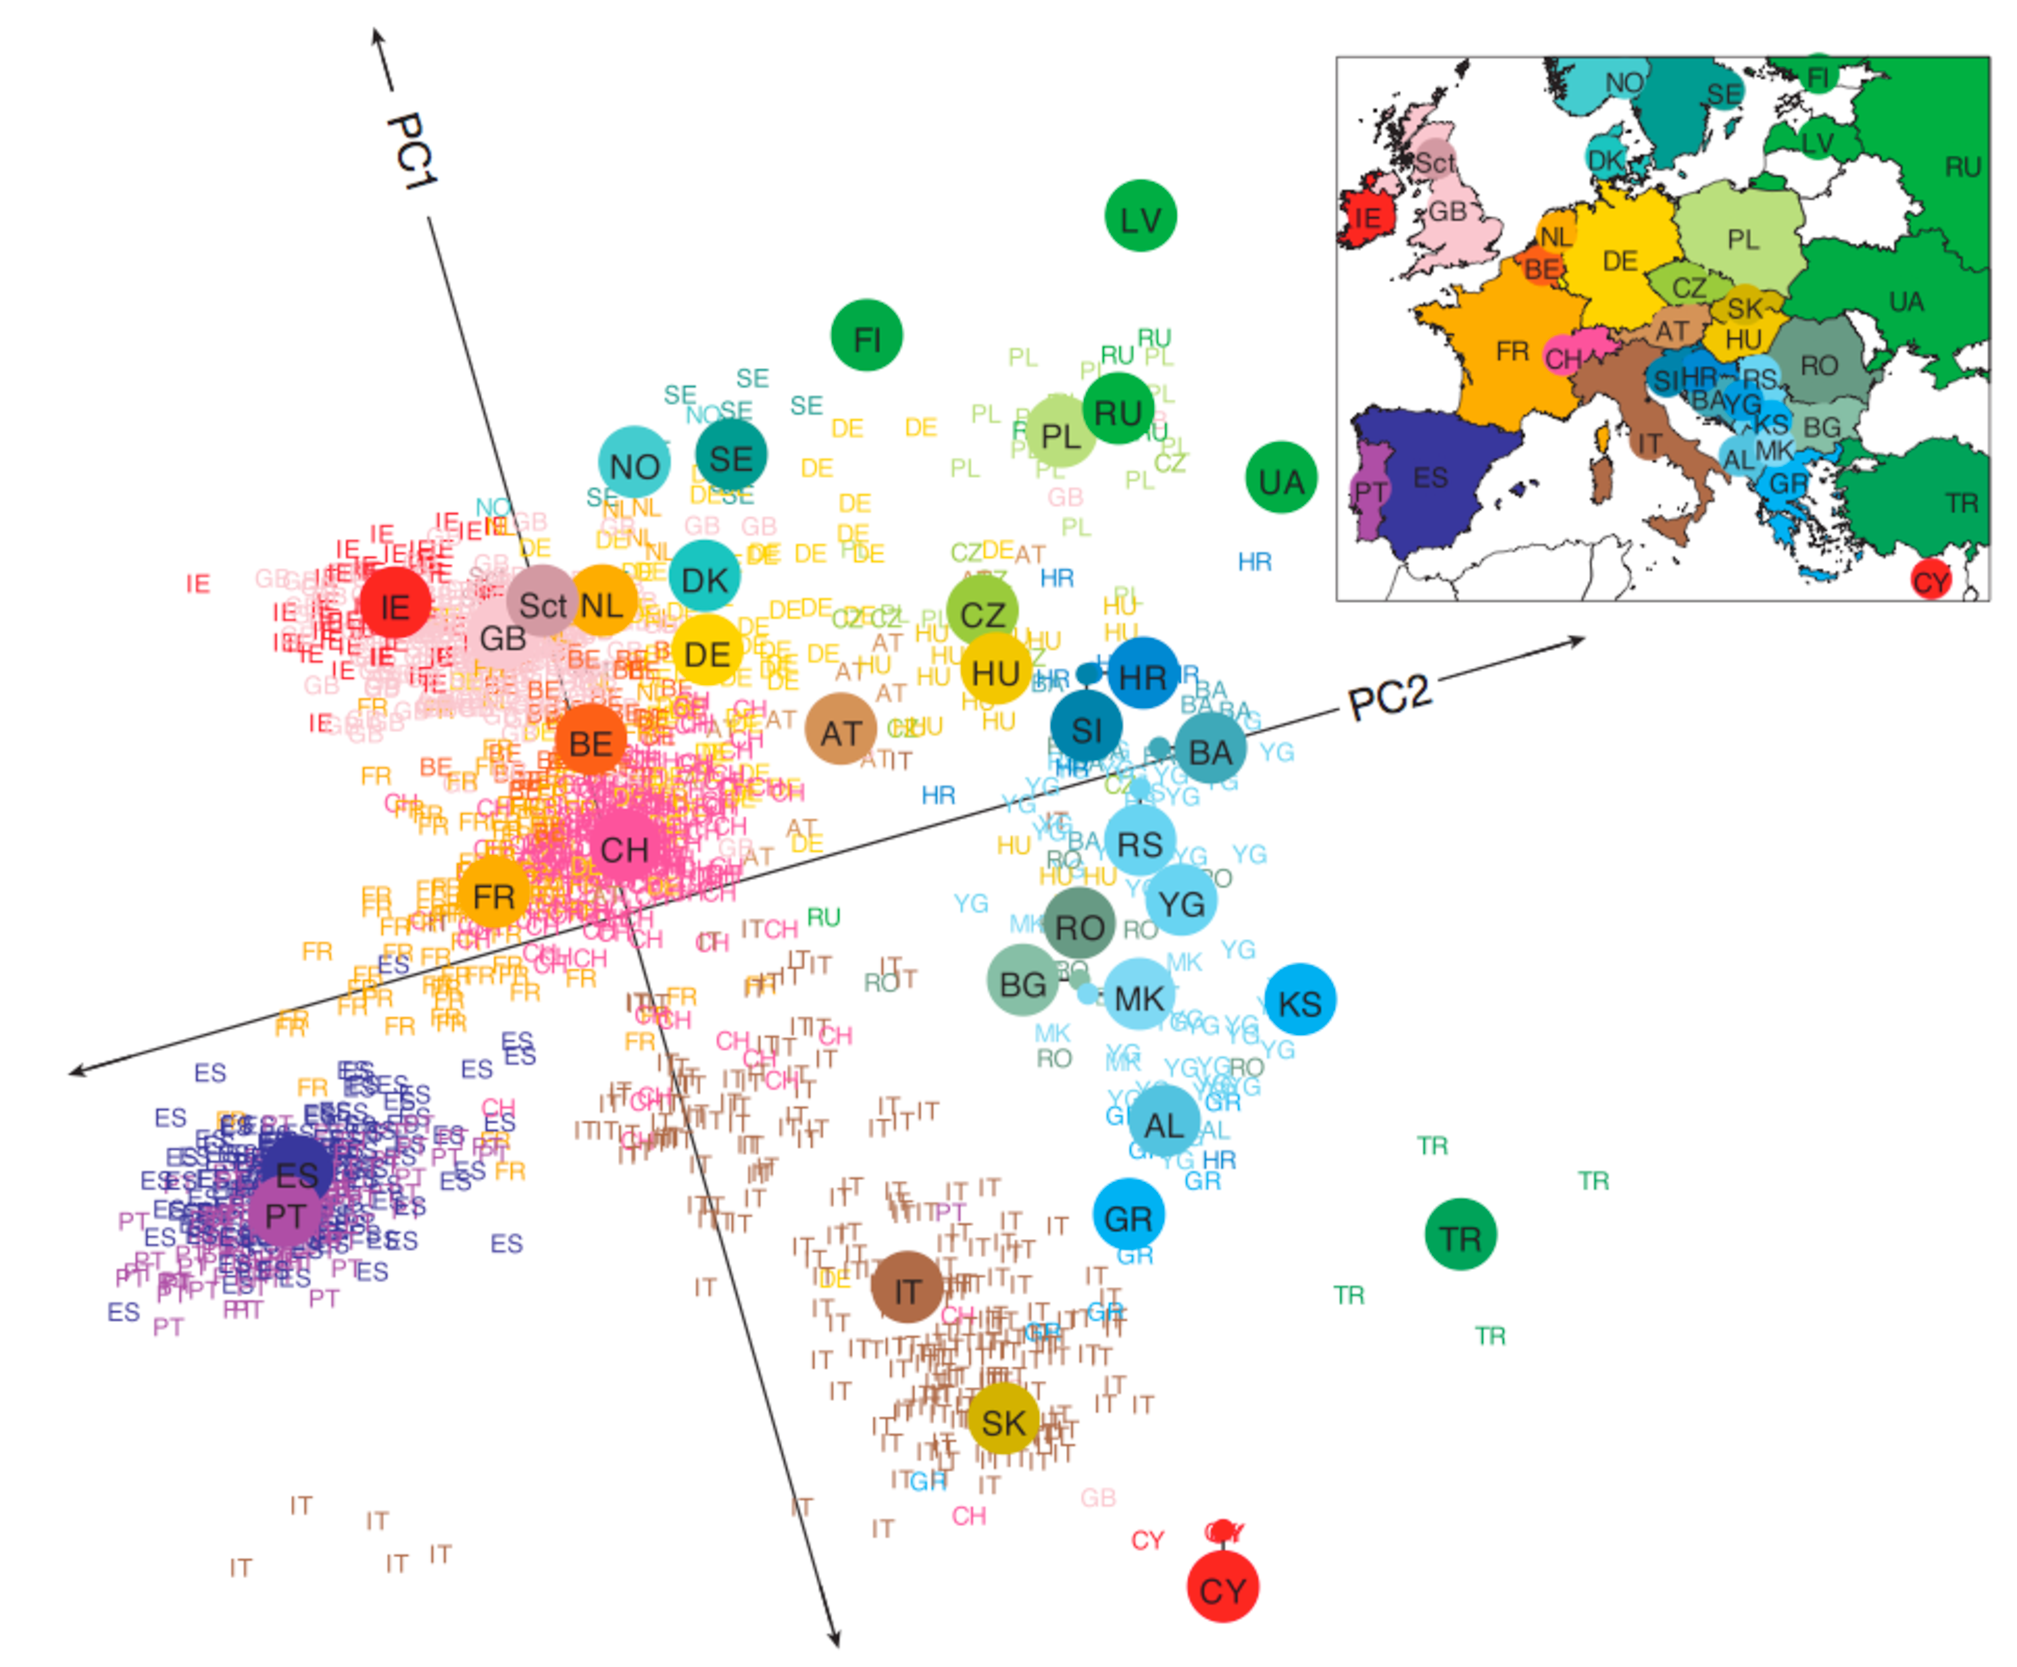
\includegraphics[width=2.8in]{../graphs/geogenes}
\end{center}
\vskip -1cm
{\tiny 
\hfill Novembre {\it et al}, Nature 456 (2008)~~~~~~~~}

\vskip .2cm
The $\bm{x}$ for each individual is a giant vector of SNPs.
They've reduced it into two factors that explain most of the variation.

\gr Turns out that location in this 2-D space looks geographical.

\vskip -.5cm
\end{frame}



\begin{frame}

\begin{columns}

\column{2.5in}



\includegraphics[width=2.8in]{../graphs/frenchman}

\column{2in}

\vskip -2cm
\hskip -2cm {\bf \theme Mixture vs Factor models}

\vskip .2cm
\hskip -2cm Factor models imply {\it mixed membership}.

\vskip .2cm

\hskip -2cm
You don't have to be {\it in} one component,

\hskip -2cm
but can be a mix of  shared latent factors.

\vskip .2cm
\gr
\hskip -2cm For example, for protein consumption\\
\hskip -1.75cm Greece could be similar to Italy in some \\
\hskip -1.75cm dimensions,  closer
to Turkey in others.

\sk\bk
So topic models were \\actually factor models!
\end{columns}

\end{frame}


\begin{frame}

{\bf \theme Topic Models: \bk factors for text}

\sk
Recall our PCA factor model: $
\ds{E}[\bm{ x}_{i}] = \bs{\varphi}_{1} v_{i1} + \ldots  \bs{\varphi}_{K} v_{iK}$.


\sk
{The bag-of-words version is a {\theme topic model}}
\[\nv
\bm{x}_i \sim \text{MN}( \omega_{i1} \bs{\theta}_1 + \ldots + \omega_{iK} \bs{\theta}_K, m)
\]
$\Rightarrow \ds{E}[\bm{x}_i/m_i] = \omega_{i1} \bs{\theta}_1 + \ldots + \omega_{iK} \bs{\theta}_K$, \\~~~~so that
$\omega_{ik}$ is like $v_{ik}$ and $\bs{\theta}_k$ is like $\bs{\varphi}_k$.


\sk
The basic interpretation is exactly the same as in PCA: 

\hfill \nv $\bs{\omega}$ is
a low-dimension version of $\bm{x}$~~~~~~~~~

\end{frame}

\begin{frame}

{\bf \theme A greedy algorithm}

\sk
Suppose you want to find the first set of factors, $\bm{v}^1 = v_{11} \ldots v_{n1}$.

We can write our system of equations (for $i=1...n$)
\[
\begin{array}{c}
\ds{E}[x_{i1}|v_{i1}] = \varphi_{11} v_{i1}\\
\vdots\\
\ds{E}[x_{ip}|v_{i1}] = \varphi_{1p} v_{i1}
\end{array}
\]
Where $\sum_{j=1}^p \varphi_{kj}^2 =1$ to nail down scale.

\vskip .1cm
The factors $\bm{v}^1$ are fit to maximize average $R^2$ in this equation.
{\gr Note that we're optimizing over both $\bs{\varphi}$ {\it and} $\bm{v}$.}

\vskip .25cm
Next, calculate residuals $e_{ij} = x_{ij}-\ds{E}[x_{ij}|v_i]$. \\
Then find $\bm{v}^2$ to maximize $R^2$ for these residuals.  

\vskip .25cm
This repeats until residuals are all zero ($\mr{min}(p,n)$ steps).

\gr
This is not actually done in practice, but the intuition is solid.
\end{frame}


\begin{frame}

{\bf A greedy algorithm for {\theme PCA}}

\sk
We're repeatedly finding {\it latent} $v_{ik}$ to {\it minimize deviance},\\ across dimensions $j=1\ldots p$ and observations 
$i=1\ldots n$,\\ for the model 
\[
e_{kij} \sim \mr{N}\left(v_{ik}\varphi_{kj},~ \sigma_k^2\right)
\]
where $e_{kij} = x_{ij} - \ds{E}[x_{ij}|v_{i1} \ldots v_{ik-1}]$ is the residual after $k-1$ factors, and we're optimizing over both 
$\bs{\varphi}_k$ {\it and} $\bm{v}^k$.


\sk
This yields principal component (PC) rotations $\bs{\Phi} = [\bs{\varphi}_1 \cdots \bs{\varphi}_K]$, with $K$ the minimum of $n$ and $p$ (i.e., where all $e_{ijK}=0$).

\sk
Think about the algorithm as repeatedly fitting regression  onto the best possible factors to explain current residuals.

\end{frame}

\begin{frame}

{\bf \theme PCA: 
{\bk projections into latent space}}

\vskip .25cm
Another way to think about factors, in our 2D example:

\vskip .25cm
\sg
PCA equivalent to finding the line that fits
through $x_1$ and $x_2$, and seeing where each observation lands
(projects) on
the line.

\vskip .25cm
~~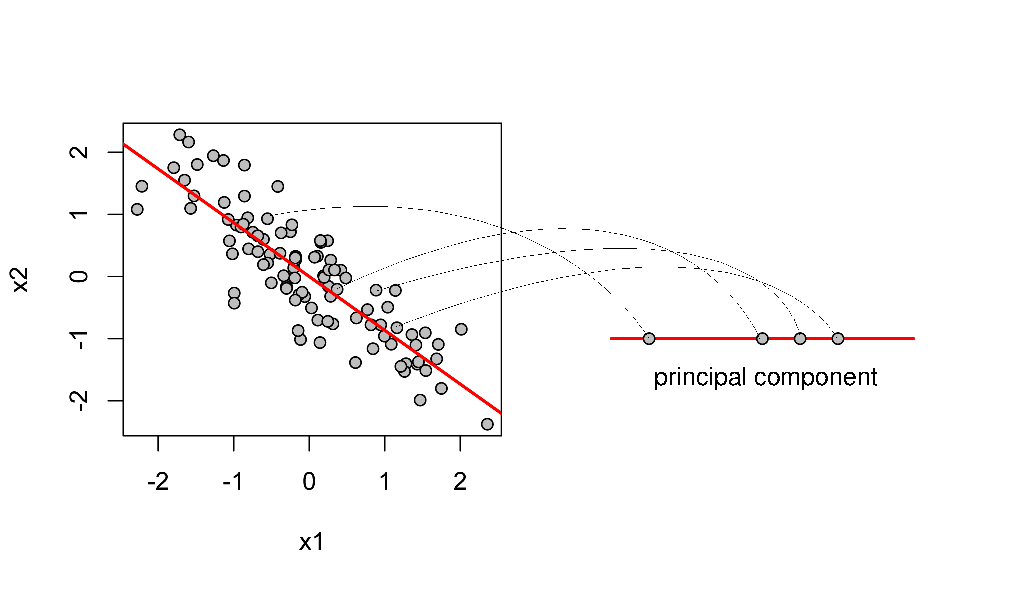
\includegraphics[width=4.25in]{../graphs/PCpath}

\gr \hfill We've projected from 2D onto a 1D axis.
\end{frame}

\begin{frame}

{\bf \theme Fitting Principal Components via \theme Least Squares}

\sk
PCA looks for high-variance projections from multivariate $\bm{x}$ 
(i.e., the long direction) and finds the least
squares fit.

\vskip -1cm
~~~~~~~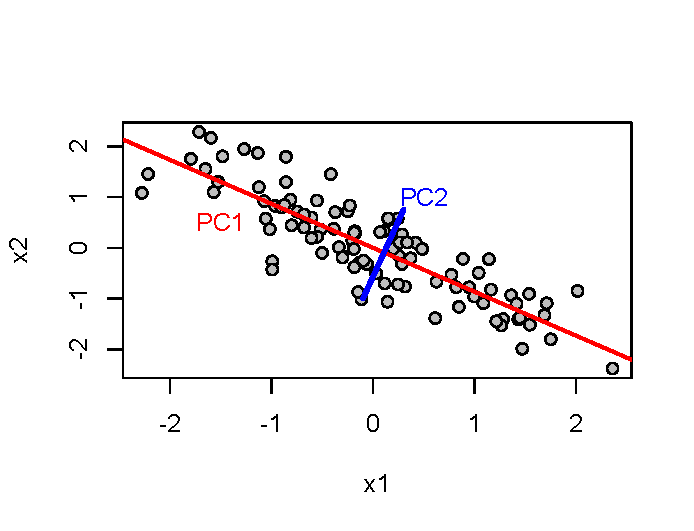
\includegraphics[width=3.5in]{../graphs/PCcomps}
\vskip -.25cm

\sg
Components are ordered by variance of the fitted projection.


\end{frame}

\begin{frame}

{\bf \theme PCA: 
{\bk Principal Components Analysis}}


\vskip .25cm
PCA fits $\ds{E}[x_{ij}]= \varphi_{j1} v_{i1} + \ldots \varphi_{jK}
v_{iK},~j=1...p$\\ by minimizing deviance over {\it both} $\bs{\varphi}$'s and $\bm{v}$'s.

\vskip .25cm
The $k^{th}$ {\theme principal component direction} for observation $i$ is
\[
z_{ki} = \bm{x}_i'\bs{\varphi}_k = \sum_{j=1}^p \varphi_{kj} x_{ij} 
\]

This is a projection from $\bm{x}$ into the space of the unknown $v_{ik}$.
$\bs{\Phi} = [\bs{\varphi}_1 ... \bs{\varphi}_K]$ are called rotations,
and we  write $\bm{z}_i = \bm{x}_i'\bs{\Phi}$.

\end{frame}



\begin{frame}

We say {\nv $x_{ij} \varphi_{jk}$ is a projection of $x_{ij}$ in
  the direction of $v_{ik}$.}\\
How does this help us simplify multivariate $\bm{x} = [x_1\dots x_p]$?


\vskip .25cm
If $x_1$ and $x_2$ are both linear functions of $v$,
then view the projection from both of them into $v$ as a single
summary.


\vskip .25cm
~~~~~~~~~~~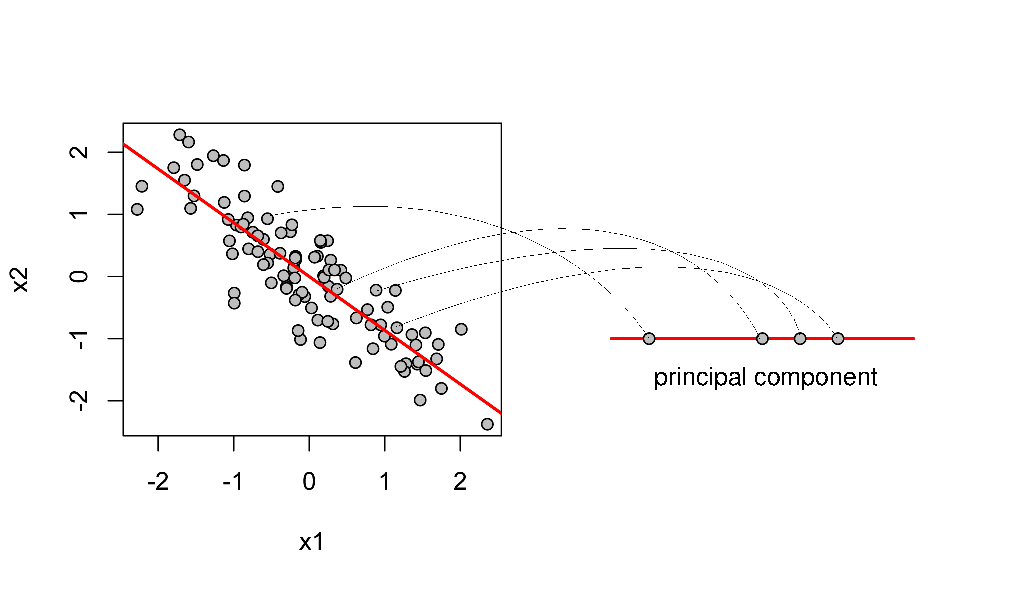
\includegraphics[width=3.5in]{../graphs/PCpath}

Instead of bothering with both $x_1$ and
$x_2$, we have a single factor that underlies both of them: $z_i = x_{i1}\varphi_1 + x_{i2}\varphi_2$.

{\gr (z is the point on the line closest to $[x_{i1},x_{i2}]$)}.

\vskip -.25cm

\end{frame}


\begin{frame}

{ Beyond geometry, the easiest interpretation is to think of each
principal component $z_{ki}$ as our best guess at 
$v_{ik}$ for new $\bm{x}_i$.}

\vskip .25cm
This occurs because of the $\sum_{j=1}^p \varphi_{kj}^2 =1$, so $z_i = \sum_{j=1}^p \varphi_{kj} x_{ij}$  is like a sum of the portions of each $x_{ij}$ related to $v_{ik}$.

\begin{center}\nv
Just think of $z_{ik} = \hat v_{ik}$, as an estimate for $v_{ik}$.
\end{center}

We work with `{\theme directions}' $\bm{z}$ rather than `{\theme factors}'
 $\bm{v}$ because this makes it easier to get PCs for new $\bm{x}$: just 
 set $\bm{z} = \bm{x}'\bs{\Phi}$.

\end{frame}

\begin{frame}

{\bf \theme Principal Components in R}

\sk
The best command to do PC is \R{prcomp(x, scale=TRUE)}.
\begin{itemize}
\item There are lots of other options; I've found prcomp solid.
\item Since we're combining least squares, it is once again good to
  {\tt scale} all the $x_j$'s to have unit variance.
\item {\tt plot(mypca)} will produce a simple screeplot.
\end{itemize}

This finds the rotations $\bs{\varphi}_1 \ldots \bs{\varphi}_p$, also
called `loadings'.  

\sk
Use {\tt predict} to access the principal components:\\
~~~~~~\R{predict(mypca)[,1:2]} gives the first two.\\
~~~~~~\R{predict(mypca, newdata=newX)} gives $\bm{z}$ for new data.

\vskip .1cm
Both of these function just multiply $\bm{x}'\bs{\Phi}$ for 
input vector $\bm{x}$.\\

{\theme NB: $\bm{x}$ is first {\it scaled} by 
the SDs used in {\tt mypca} if {\tt scale=TRUE}.}



\end{frame}


\begin{frame}[fragile]

{\bf \theme  Understanding Principal Components}

\sk

Given (say) 4 factors, country `$i$' has expected \\protein consumption 
$ v_{i1} \bs{\varphi}_1 +  v_{i2} \bs{\varphi}_2 +  v_{i3} \bs{\varphi}_3 + v_{i4} \bs{\varphi}_4$.

\vskip .2cm{\nv
We can interpret each $v_{ik}$ as a `diet factor': a way of eating.}

\vskip .2cm
Rotations $\bs{\varphi}_k = [\varphi_{k,rm} \cdots \varphi_{k,fv}]$ 
{\gr ($rm$:
  red meat, $fv$: fr/veg)}
thus encode the {\it foods} associated with diet $k$.



\sk
The $k^{th}$ principal component for each country
\[
z_{ik} = \sum_{j=1}^p x_{ij}\varphi_{kj} = 
x_{i,rm} \varphi_{k,rm} + \ldots
+ x_{i,fv} \varphi_{k,fv} 
\]
is then a score for how much $i$'s consumption matches diet $k$.

\end{frame}

\begin{frame}[fragile]

{\theme  loadings as diet:}
use rotations on interpretable $x_j$ to build
a story for the latent factor space.  This can be tough!

\vskip .25cm
Note that if you fit {\tt prcomp} with {\tt scale=TRUE}, the {\tt rotation} matrix
is on the scale of standard deviations:  \\ ~~~{\theme $\varphi_{jk}$ is units of direction $z_k$ gained for a 1 sd increase in $x_j$.}

{\gr These `units' are not easily interpretable, but we try.}


\sk
 Rotations {\gr ($\bs{\varphi}_k$) } for the first two food factors:\\

{\nv \footnotesize
\begin{verbatim}
> t(round(pcfood$rotation[,1:2],2))
   R.Meat W.Meat  Eggs  Milk  Fish Cereal Starch Nuts Fr.Veg
PC1 -0.30  -0.31 -0.43 -0.38 -0.14   0.44  -0.30 0.42   0.11
PC2 -0.06  -0.24 -0.04 -0.18  0.65  -0.23   0.35 0.14   0.54
\end{verbatim}}

PC1 is high nut/grain, low meat/dairy. \\PC2 is Iberian:
move 0.65 in that direction with 1sd extra {\theme fish}.
\end{frame}


\begin{frame}[fragile]

{\bf Understanding the principal components}

\sk How many do we need?  What do the factors contribute?

{\nv \footnotesize
\begin{verbatim}
> summary(pcfood)
Importance of components:
                          PC1    PC2    PC3    PC4     PC5
Standard deviation     2.0016 1.2787 1.0620 0.9771 0.68106
Proportion of Variance 0.4452 0.1817 0.1253 0.1061 0.05154
Cumulative Proportion  0.4452 0.6268 0.7521 0.8582 0.90976
\end{verbatim}}

The summary tells us what {\tt cumulative proportion} of variation is explained
by the factors $1 ... K$.

\vskip .2cm
Each PC's contribution to this is decreasing with its variance.

\end{frame}

\begin{frame}

{\bf {\theme Screeplot:} show variance for each principal component.}

\vskip -.5cm
\hskip .5cm 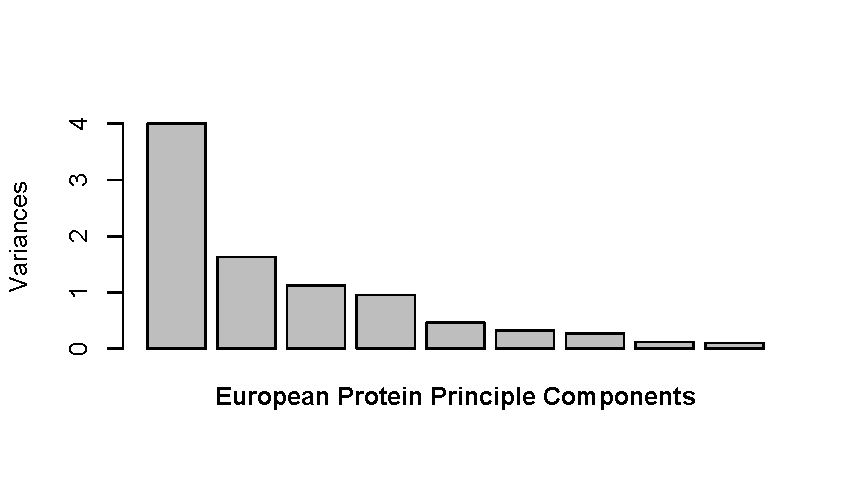
\includegraphics[width=4in]{../graphs/FOODscree}

\vskip -.5cm

PC with high var($z_k$) are useful to differentiate
observations.\\{\gr
The directions are uninteresting once variance levels out, and
After a subjective threshold, we consider the PC ``just noise''.}


\vskip .2cm
{\nv Screeplots are heavily used, but barely useful.}
Here, it actually looks to me like only the first really matters. 
However...

\vskip -.5cm
\end{frame}


\begin{frame}


{\bf Principal components in {\theme  European protein consumption}}

\vskip -.5cm
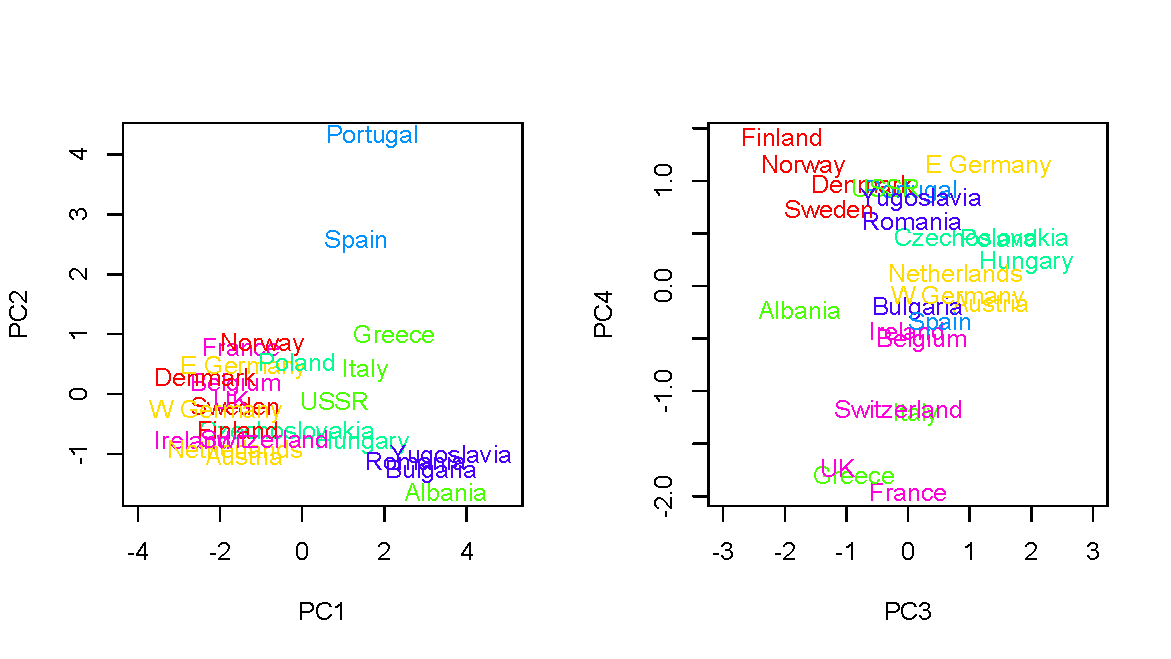
\includegraphics[width=4.25in]{../graphs/FOODpc}

Overlaying  k-means clustering from week 5, we see that\\ the
nation-groups are far apart in the first 4 PC directions.

\vskip .2cm
Like in any other purely unsupervised model, the goal is exploration and 
intuition. {\nv So use a $K$ that makes sense to you.}


\end{frame}


\begin{frame}

\begin{columns}

\column{3.5in}

~~~~~{\bf Congress and \theme Roll Call Voting}

\sk\sg
~~~~~Votes in which names and positions \\~~~~~are recorded are called `roll calls'.

\sk\gr
~~~The site {\tt voteview.com} archives vote records\\
~~~and the R package { \tt pscl} has tools for this data.

\sk\sg
~~445 members in the last US House 
(the $111^{th}$)\\
~~1647 votes: 
\theme nea = -1, \nv yea=+1, \gr missing = 0.

\sk\bk
This leads to a large matrix of observations that can probably be
reduced to simple factors {\gr (party)}.


\column{1in}
 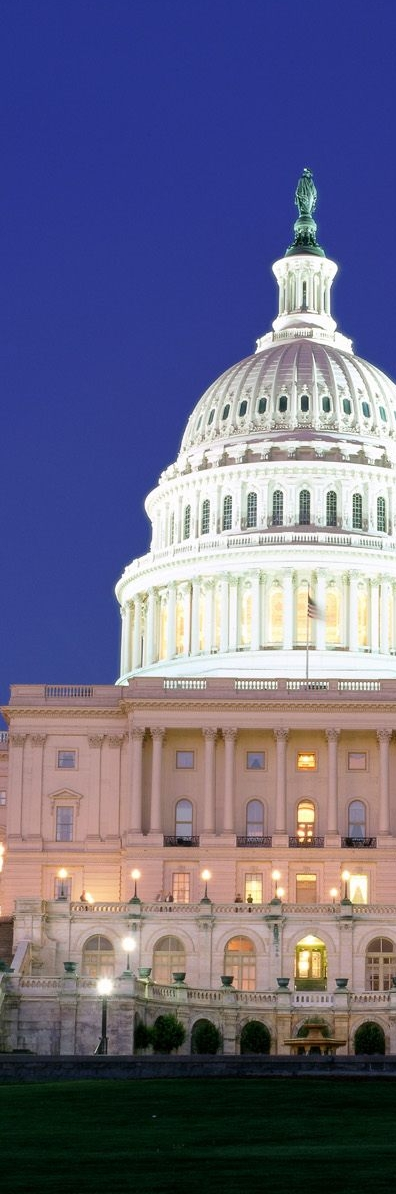
\includegraphics[width=1.25in]{../graphs/USCongress}
\end{columns}
\end{frame}


\begin{frame}

{\bf \theme Vote components in the $\bs{111^{th}}$ house}

\sk
\hfill The model is $\ds{E}[\bm{x}_i] =v_{i1} \bs{\varphi}_1 + v_{i2}
\bs{\varphi}_2 + \ldots$\\
\hfill Each PC is $z_{ik} = \bm{x}_i\bs{\varphi}_k = \sum_j x_{ij}\varphi_{kj}$~~
\vskip -2cm
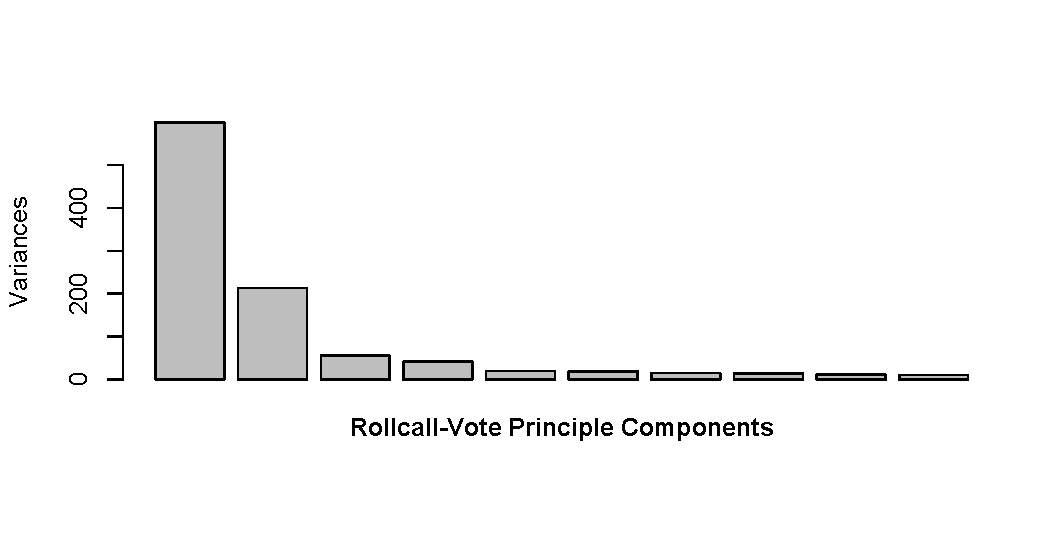
\includegraphics[width=4.5in]{../graphs/VOTEscree}

\vskip -.5cm
\gr Huge drop in variance from $1^{st}$ to $2^{nd}$ and  $2^{nd}$ to $3^{rd}$ PC.

\vskip .5cm
\bk
Poli-Sci holds that PC1 is usually enough
to explain congress. \\\sg 2nd component has been important twice: 1860's and 1960's.
\end{frame}


\begin{frame}

~~~~~~~~~~~~~{\bf Top two PC directions in the $\bs{111^{th}}$ house}

\vskip -1cm

\hskip .3cm 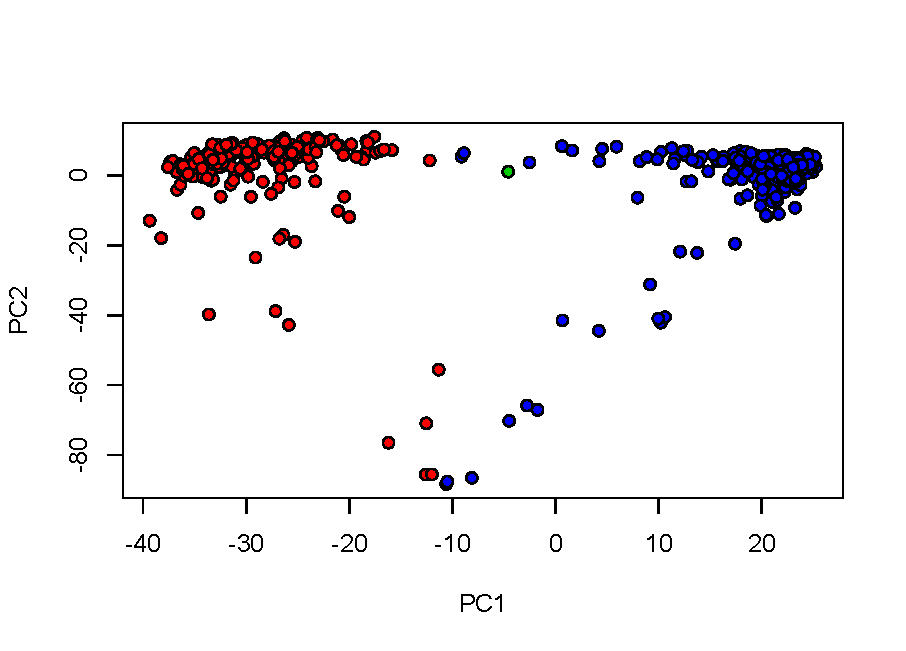
\includegraphics[width=4in]{../graphs/VOTEpc}

\vskip -.25cm
\sg
Republicans in red and Democrats in blue: 
\begin{itemize}\gr
\item Clear separation on the
first principal component.
\item
The second component looks orthogonal to party.
\end{itemize}

\vskip -.5cm

\end{frame}

\begin{frame}[fragile]

{\bf Interpreting the principal components}

\sk
{\scriptsize \nv

{\theme \tt \#\# Far right (very conservative) \vspace{-.25cm}}
\begin{verbatim}
> sort(votepc[,1])
     BROUN (R GA-10)       FLAKE (R AZ-6)   HENSARLIN (R TX-5) 
         -39.3739409          -38.2506713          -37.5870597 
\end{verbatim}

{\theme \tt \#\# Far left (very liberal) \vspace{-.25cm}}
\begin{verbatim}
> sort(votepc[,1], decreasing=TRUE)
    EDWARDS (D MD-4)   PRICE (D NC-4)    MATSUI (D CA-5)      
         25.2915083        25.1591151         25.1248117     
\end{verbatim}       
  

{\theme \tt \#\# social issues? immigration? no clear pattern\vspace{-.25cm}}
\begin{verbatim}
> sort(votepc[,2])
     SOLIS (D CA-32) GILLIBRAND (D NY-20)      PELOSI (D CA-8) 
        -88.31350926         -87.58871687         -86.53585568 
   STUTZMAN (R IN-3)       REED (R NY-29)      GRAVES (R GA-9) 
        -85.59217310         -85.53636319         -76.49658108 
\end{verbatim}
}

\gr PC1 is easy to read, PC2 is ambiguous (is it even meaningful?)
\end{frame}


\begin{frame}

{\bf \nv High PC1-loading votes are \theme  ideological battles.} 
\\These tend to have  informative
voting across party lines.

\vskip -.5cm
\hskip .3cm 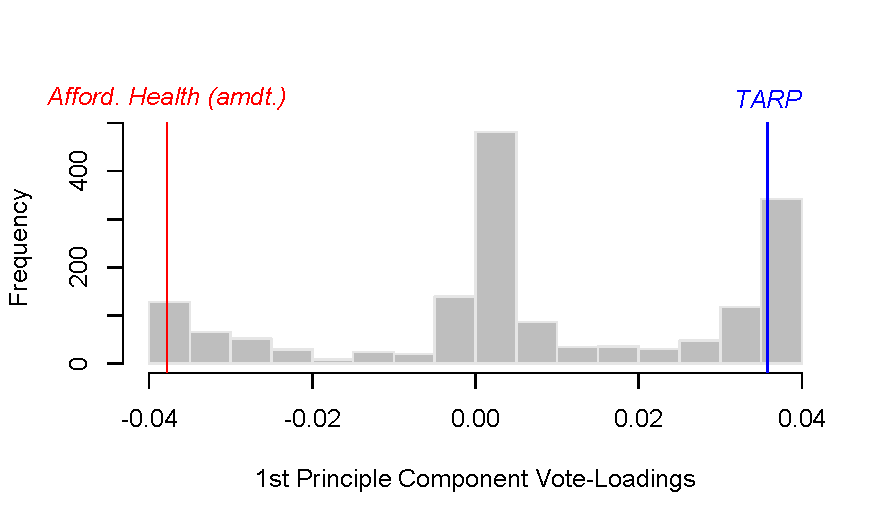
\includegraphics[width=4in]{../graphs/VOTEloads}

 \footnotesize \sg
A vote for Republican amendments to `Affordable Health
Care for America' strongly indicates a negative PC1
(more conservative), while \\a vote for TARP indicates a positive PC1
(more progressive).

\end{frame}


\begin{frame}[fragile]


\sg  
Look at the largest loadings in $\bs{\varphi}_{2}$ to discern an
interpretation.

{\nv \scriptsize 
\begin{verbatim}
  > loadings[order(abs(loadings[,2]), decreasing=TRUE)[1:5],2]
   Vote.1146   Vote.658  Vote.1090  Vote.1104  Vote.1149 
  0.05605862 0.05461947 0.05300806 0.05168382 0.05155729 
\end{verbatim} }
  
\vskip -.25cm
These votes all correspond to near-unanimous  symbolic
action.

\vskip .25cm
\bk
For example, 429 legislators voted for resolution 1146: \\
`{\sg Supporting the goals and ideals
  of a Cold War Veterans Day}'\\\hfill
{\gr If you didn't vote for this, you weren't in the house.}


\sk {{\theme Mystery Solved: } the second PC is just attendance!}
\vspace{- .1cm}
{\nv \scriptsize 
\begin{verbatim}
 > sort(rowSums(votes==0), decreasing=TRUE)
      SOLIS (D CA-32) GILLIBRAND (D NY-20)       REED (R NY-29) 
                 1628                 1619                 1562 
    STUTZMAN (R IN-3)      PELOSI (D CA-8)      GRAVES (R GA-9) 
                 1557                 1541                 1340 
\end{verbatim}}
\vspace{- .25cm}

\end{frame}

\begin{frame}[fragile]

{\bf \theme PCR: \bk Principal Component Regression}

\vskip .25cm
The concept is very simple: instead of regressing onto $\bm{x}$, use
a lower dimension set of principal components $\bm{z}$ as covariates.

\vskip .25cm
This works well for a few reasons:
\begin{itemize}
\item PCA reduces dimension, which is always good.
\item Higher variance covariates are good in regression, \\and we choose
  the top PCs to have highest variance.
\item The PCs are independent: no multicollinearity.
\end{itemize}

\vskip .25cm
The 2-stage algorithm is straightforward.
For example,

{\nv 
\begin{semiverbatim}\vspace{-.25cm}\small
         mypca = prcomp(X, scale=TRUE)
         z = predict(mypca)[,1:K]
         reg = glm(y~., data=as.data.frame(z))
\end{semiverbatim}
}

\vspace{-.25cm}
For new data, \small
{\tt\nv znew = predict(mypca,xnew)[,1:K] \\ \hskip 1cm pred = predict(reg,as.data.frame(znew))}.


\end{frame}

\begin{frame}


\begin{columns}

\column{1.7in}

~~
\includegraphics[width=1.75in]{../graphs/television}

\column{3in}

Data from NBC on response to TV pilots

\vskip .15cm
 \gr 6241 views and 20
questions for 40 shows

\vskip .15cm
\sg Primary goal is predicting {\theme engagement}.

\end{columns}

\sk
Classic measures of broadcast marketability are {\theme Ratings}.\\
{\nv GRP}: \gr gross ratings points; estimated total viewership.\\
{\nv TRP}: targeted ratings points; viewership in specific categories.

\sk\bk
{\theme Projected Engagement:} a more subtle measure of
audience.\\
\gr After watching a show, viewer is quized on order and detail.\\
\sg This measures their engagement with the show (and ads!).

\end{frame}



\begin{frame}

{\theme \bf Predicting TV Engagement with PCR}

\vskip .25cm
Engagement matters for GRP, and also in adjusted GRP/PE.

\vskip -.5cm
~~~~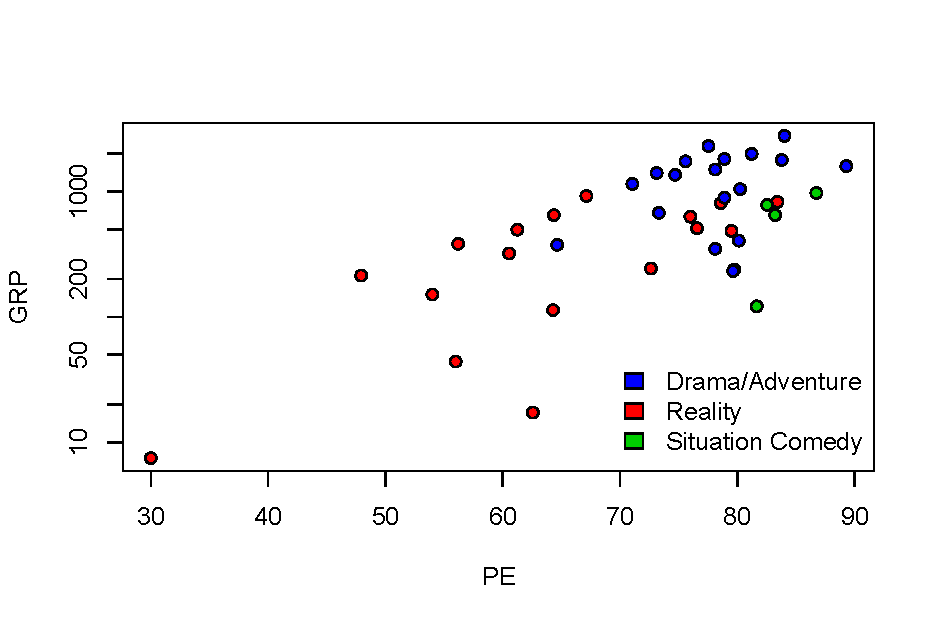
\includegraphics[width=3.5in]{../graphs/NBCshows}


\vskip -.25cm
Given the survey responses and eventual projected engagement (PE), can we
find a low-D model for predicting engagement from survey
response in pilot focus
groups?

\end{frame}



\begin{frame}[fragile]

{\theme \bf NBC Pilot-Survey PCA}

\begin{columns}
\column{1.7in}
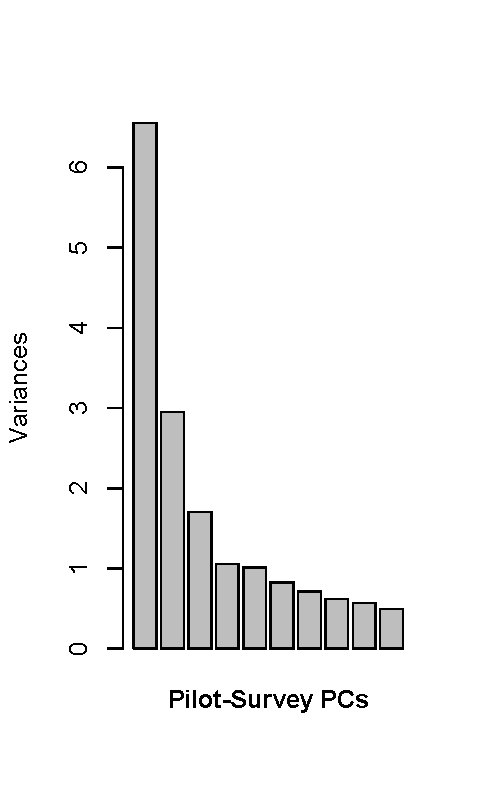
\includegraphics[width=1.7in]{../graphs/NBCscree}

\column{2.4in}{\nv \footnotesize
\begin{verbatim}
> round(PCApilot$rotation[,1:3],1) 
                 PC1  PC2  PC3
Q1_Excited      -0.3  0.1 -0.1
Q1_Happy        -0.1  0.2 -0.5
Q1_Engaged      -0.3  0.0  0.0
Q1_Annoyed       0.2  0.3  0.1
Q1_Indifferent   0.2  0.4  0.1
Q2_Funny         0.1  0.2 -0.5
Q2_Confusing    -0.1  0.3  0.2
Q2_Predictable   0.2  0.3  0.0
Q2_Entertaining -0.3 -0.1 -0.3
Q2_Original     -0.3  0.1 -0.2
Q2_Boring        0.2  0.4  0.1
Q2_Dramatic     -0.2  0.0  0.4
Q2_Suspenseful  -0.3  0.0  0.3
\end{verbatim}
\sk
}

\end{columns}

Huge drop after the first PC, but a few could be influential.\\
How do questions load? Maybe these are three genres...


\end{frame}

\begin{frame}

{\bf NBC Pilot-Survey Principal Components}

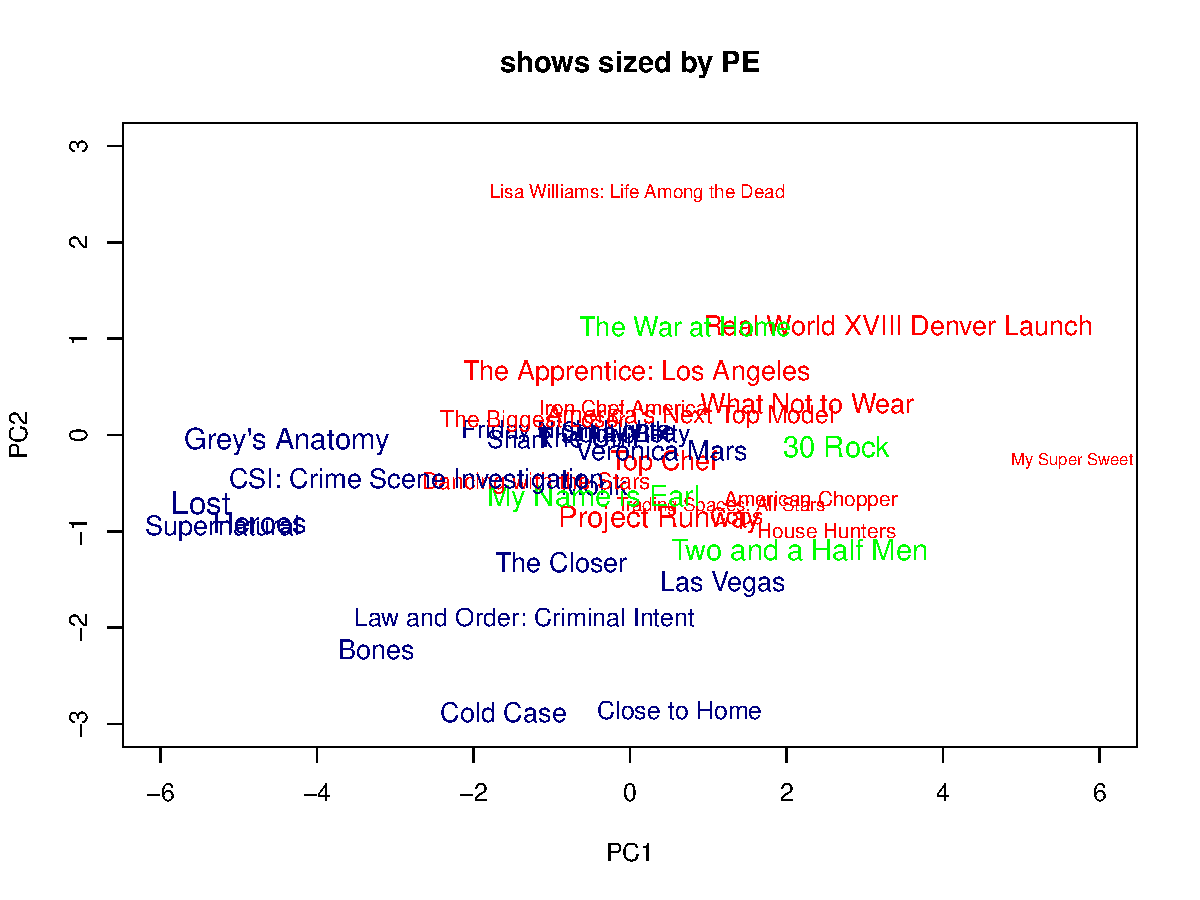
\includegraphics[width=4in]{../graphs/NBCpilotavgPCs}


We first aggregated responses by show, then fit PC.

\end{frame}



\begin{frame}

{\bf  \theme Choosing the number of factors}

\sk
Like in $K$-means, this is tough without supervision.

\vskip .05cm
For PCR, though, we can just use the usual tools.

\vskip .05cm
There are two ways to do this

\vskip .1cm
\begin{enumerate}
\item Regress onto factors 1 through $K$ for a few $K$, 
  and choose the model with lowest IC or CV error.
\item Lasso all $p$ factors with $\lambda$ selected via IC or CV.
\end{enumerate}

\vskip .25cm
Both are fine.  

\end{frame}



\begin{frame}

{\bf \nv Factor selection for NBC pilot survey}

\vskip -.5cm
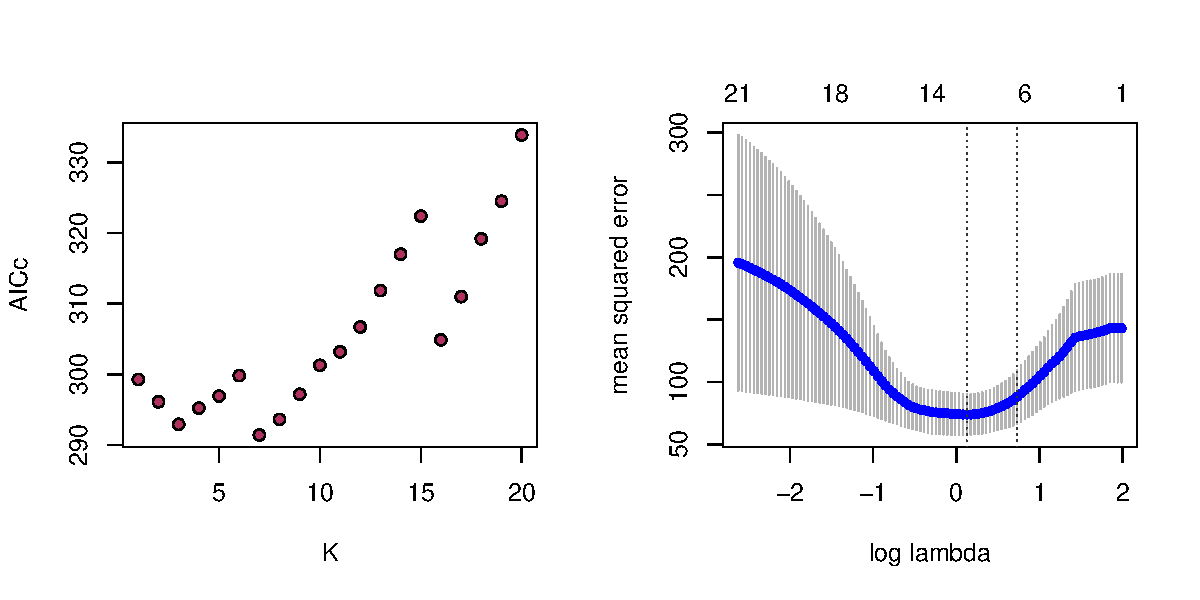
\includegraphics[width=4.25in]{pilotPEselect}

\vskip -.25cm
AICc building one-at-a-time chooses $K=7$, \\but the curve is all over the place.

\vskip .1cm
CV lasso chooses the first three plus a couple others.

\end{frame}



\begin{frame}

{\bf \theme Factor Models \bk vs \theme Variable Selection}

\vskip .25cm
Both are good tools; you can mix and match as needed.\\
What to use often comes down to preference and experience.

\vskip .25cm
PCA/PCR is nice in social science because you\\get
latent structure (e.g., the `partisan factor').  \\{\gr But sometimes this is
 imaginary, so be careful.}

\sk 
{\bf \nv Sparse \bk vs \nv Dense \bk regression models}
  
\vskip .25cm More conceptually, lasso finds a {\it sparse} model 
(many $\beta_j=0$), whereas PCR assumes all the $x$'s matter but only through the information they provide on a few simple factors.

%\vskip .1cm{\gr Even lasso-PCR is dense in $\bm{x}$ (it is sparse in $\bm{z}$).}

\vskip .25cm  Both do dimension reduction! \\Which is best will depend upon the application.

\vskip -.5cm
\end{frame}

\begin{frame}
{EXTRA: supervised factors}

An issue we discussed with clustering is relevant here too:

\vskip .1cm
Factor model regression (e.g., PCR) will only work if the dominant directions of variation in $\bm{x}$ are related to $y$.

\vskip .5cm
Is there a way to force factors $\bm{v}$ to be relevant to both $\bm{x}$ and $y$?  

\vskip .1cm
\hfill Yes, and its a nice Big Data technique.

\end{frame}

\begin{frame}

{\bf \theme Marginal Regression}

\sk
An old idea
\begin{itemize}
\item Calculate $\bs{\varphi} = [\varphi_1 \ldots \varphi_p] 
= \mr{cor}(\bm{x},y)/\mr{sd}(\bm{x})$.
\item Set $z_i = \bm{x}_i'\bs{\varphi} = \sum_{j} x_{ij}\varphi_j$.
\item Fit the simple linear regression $y \sim z$.
\end{itemize}

\sk
Marginal Regression is a natural for MapReduce.
\begin{itemize}
\item Map data to $n\times 2$ {\tt \{ x[i,j],y[i] \} } matrices.
\item Send each matrix to a reducer for calculating $\varphi_j$.
\item In a 2nd MapReduce step, 
map each $\bm{x}_i$ and reduce $\bm{x}_i'\bs{\varphi}$
\item Finally, just fit OLS $\ds{E}[y_i|z_i] = \alpha + \beta z_i$.
\end{itemize}
{ For this reason, MR is having a comeback.}

\end{frame}


\begin{frame}


\begin{columns}

\column{2.2in}

{\bf   ~~~~~Example: Gas Data}

\vskip .25cm
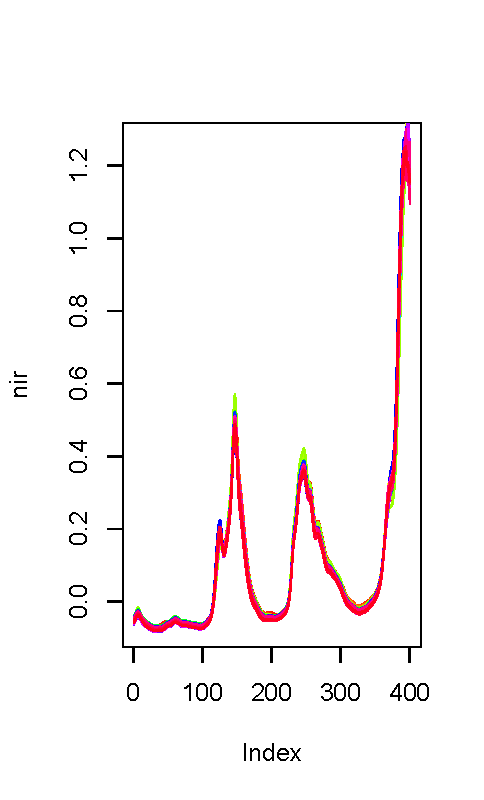
\includegraphics[width=2in]{../graphs/gasplot}

\column{2.7in}

\sk
When you buy gas,\\it has an octane (quality) rating.  \gr\\
This is measured  through failure \\testing on a
model engine.

\sk\bk
More frequent testing is possible through NIR sensors:
\begin{itemize}
\item Near infrared Spectroscopy measures reflectance at
  wave-lengths (1700 here)\\ longer than visible light.
\item It is useful for determining\\ chemical composition
\end{itemize}


\end{columns}

\end{frame}


\begin{frame}[fragile]

{\nv \bf Marginal Regression}

\sk

The model is 
$ \theme \ds{E}[\bm{ x}_{i}/\mr{sd}(\bm{x})] = \bs{\varphi}y_i $.

\vskip .1cm
Marginal `direction' is $\theme z_i =
\sum_j x_{ij} \mr{cor}(x_j,y)/\mr{sd}(x_j)$

\vskip .1cm
And the `forward regression model' is $\theme \ds{E}[y_i \mid \bm{x}_i] = \alpha +
\beta z_i$
\sk


\begin{columns}
\column{2.5in}

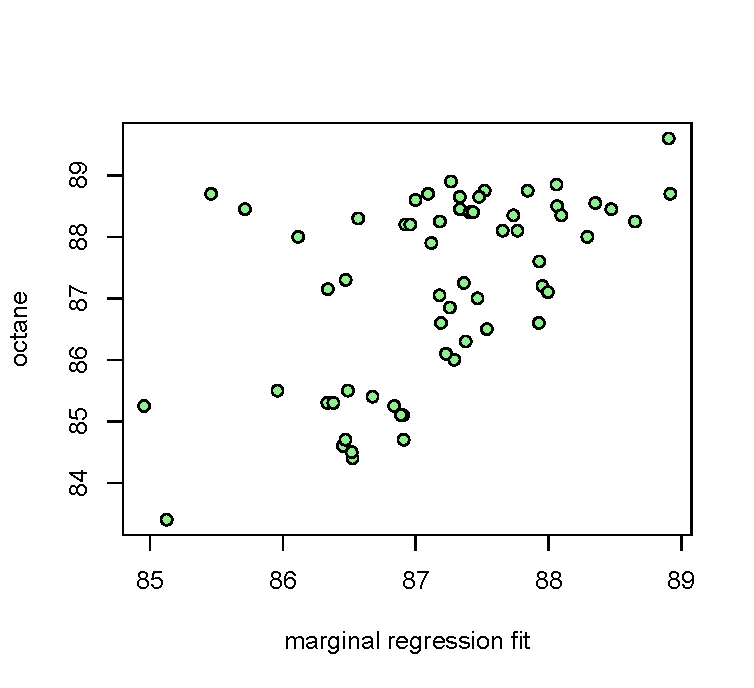
\includegraphics[width=2.5in]{../graphs/gasfit}

\column{2in}

{\nv \footnotesize \vspace{-1.5cm}
\begin{verbatim}
### marginal regression
r <- cor(nir, octane)
s <- apply(nir,2,sd)
phi <- r/s
z <- nir%*%phi
fwd <- glm(octane ~ z)
\end{verbatim}}

\end{columns}

\vskip -1cm
{\gr \hfill $R^2 \approx 30\%$~~~~~~~~~~~~}

\end{frame}


\begin{frame}[fragile]

\label{pls}

{\bf \theme  PLS: \bk Partial Least Squares}

\sk

Repeated marginal regressions to 
overcome  `marginalness'
\begin{itemize}
\item  PLS starts with $v_{i1} = y_i $.
\item  fits
$\bs{\varphi}_{1}$ for marginal regression.
\item  then iteratively sets $v_{ik}$
to residuals from the \\regression $\ds{E}[y] = \alpha+ \beta_1z_1
+\ldots+ \beta_k z_k$.
\end{itemize}
{ $z_k = \sum_j x_{ij} \varphi_{jk}$ is the $k$th PLS direction}

\vskip .25cm
\bk Recursively fit residuals onto covariates:  stage-wise regression.

\vskip .25cm
Since you just keep feeding back residuals, you can repeat \\this to get
as good a fit as desired: {\theme it is easy to overfit!}


\end{frame}



\begin{frame}[fragile]

{\bf Gas Data {\theme PLS(4)} Fit}

\sk
\R{textir} has a pls function, along with \R{summary}, \R{plot}, etc.


Get predictions with, e.g.,
\nv
\verb=predict(gaspls, nir)=


\nv
\begin{verbatim}
gaspls <- pls(X=nir, y=octane,  K=4)
\end{verbatim}

\vskip -.5cm
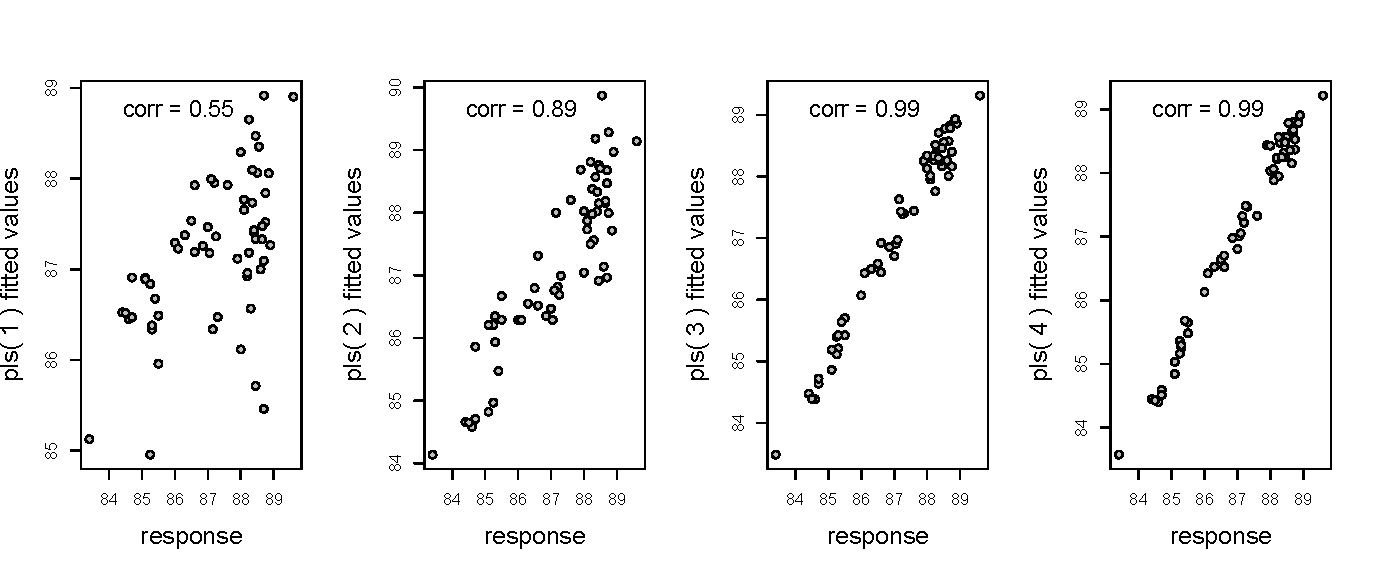
\includegraphics[width=4.25in]{../graphs/GASpls}


{\gr Note: {\tt pls(1)} is just marginal regression}

\end{frame}


\begin{frame}[fragile]
{Foreign Exchange}

{What are the latent factors of international currency pricing?}

And how do these factor move against US equities?

\vskip .25cm
We're going
to investigate underlying factors in currency exchange rates and regress
the S\&P 500 onto this information.  

\vskip .25cm FX data is in \R{FXmonthly.csv}.  

\vskip .1cm
SP500 returns are in \R{sp500csv}.

\vskip .1cm
Currency codes are in {\nv\tt currency\_codes.txt}.

\vskip .25cm

{Translate the prices to `returns' via
\begin{semiverbatim}\vspace{-.25cm}\nv
fx <- read.csv("FXmonthly.csv")
fx <- (fx[2:120,]-fx[1:119,])/(fx[1:119,]) 
\end{semiverbatim}}

\end{frame}

\begin{frame}
{Homework Due Next Week}


[1] Discuss correlation amongst dimensions of {\tt fx}.  \\How does this relate to the applicability of factor modelling?

\vskip .2cm
[2] Fit, plot, and interpret principal components.

\vskip .2cm
[3] Regress SP500 returns
onto currency movement factors, using both `{\tt glm} on first $K$' and lasso techniques. \\Use the results to add to your factor interpretation.

\vskip .2cm
[4] Fit lasso to the original covariates and \\~~~describe how it differs from PCR here.

\vskip .2cm
{\gr [+] Fit marginal regression and PLS and compare to PCA.}

\end{frame}


\end{document}
